%DAN:
%1) You need a readme, and a main.R
%2) You need a header on each of your scripts
%3) You've explored a reasonable number of models, and some do quite well
%4) A bit sloppy in places, especially with the lost code
%5) Pretty wild that your simplest model did better than even the transfer learning. Surprising,
%but I don't see anything wrong with that result. 
%6) Some places in the write up appear distinct from the code, e.g., in the writeup it says
%you use just 100 images per category but I don't see that in the code.
%Grade: S

\documentclass{article}
\usepackage[utf8]{inputenc}
\usepackage{graphicx}
\usepackage{geometry}
\geometry{margin=1in}
\usepackage{float}


\title{Neural Network Write Up}
\author{Alex Hey}
\date{\today}

\begin{document}

\maketitle

\section*{Objective}
Today's goal was to preprocess a **thinned dataset** of image data (limited to 100 images per category), train a neural network using Keras, and evaluate its performance. The dataset consisted of three categories: **cats**, **dogs**, and **snakes**.

\section*{Dataset Preparation for Day01}
To reduce complexity:
\begin{itemize}
    \item Only 100 images per category were loaded.
    \item Labels were assigned to correspond to categories: cats (0), dogs (1), and snakes (2).
    \item For Day 2, 500 images were used to thin the dataset
\end{itemize}

\section*{Day 1: Initial Model Training}

\subsection*{Original Model}
The first model used the \texttt{sparse\_categorical\_crossentropy} loss function with a dropout rate of 0.5. Below is the accuracy plot:

\begin{figure}[h!]
    \centering
    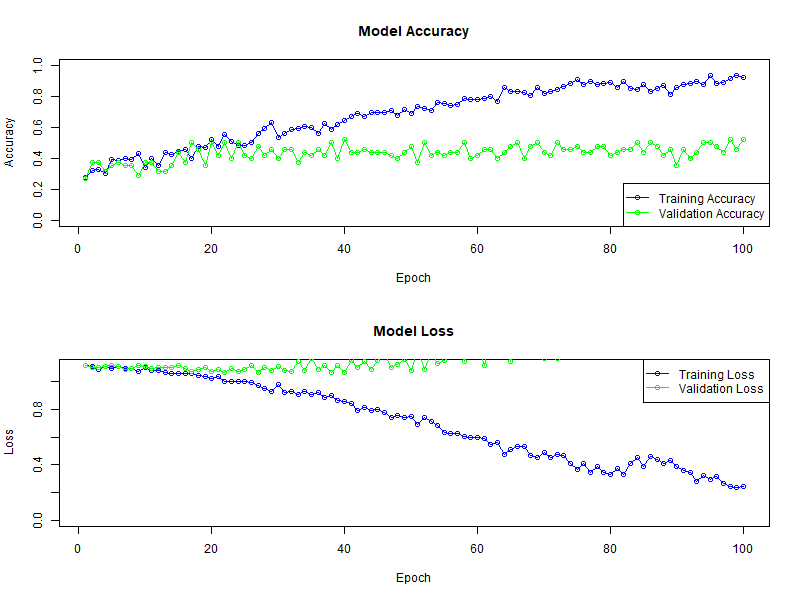
\includegraphics[width=0.6\textwidth]{../results/training_plots.png}
    \caption{Day 1: Original Model Accuracy Over Epochs (Sparse Categorical Crossentropy)}
\end{figure}

This model did not perform well. Validation accuracy never got to a point where it wa smuch better than a random guess, which would be about 30 percent accuracy. Further tuning of dropout rates or experimenting with a different loss function might improve performance.

\section*{Day 2: Modified Models}

\subsection*{Model 1: Reduced Dropout Rate}
This model decreased the dropout rate from 0.5 to 0.3, \\
while keeping the loss function as \texttt{sparse\_categorical\_crossentropy}.
Below is the accuracy plot:

\sloppy
This adjustment was made to test if a lower dropout rate would reduce overfitting. I also altered the image processing before to do 500 images per category.
\sloppypar

\begin{figure}[h!]
    \centering
    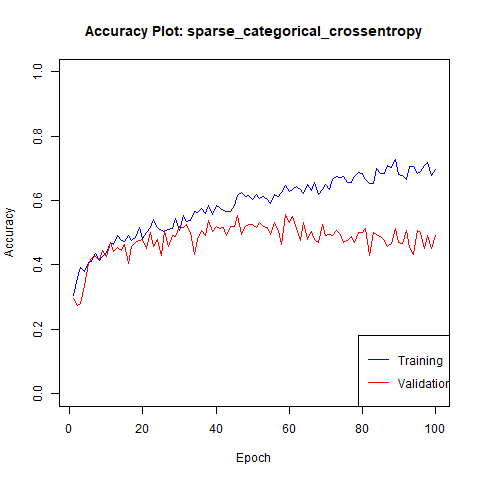
\includegraphics[width=0.8\textwidth]{../results/sparse_categorical_crossentropy_accuracy_plot.png}
    \caption{Model 1: Reduced Dropout Rate Accuracy Over Epochs (Sparse Categorical Crossentropy)}
\end{figure}

This model showed some improvement in training accuracy but struggled with validation accuracy with that only improving slightly from the previous model. The next model will change the loss function to see if that helps:

\subsection*{Model 2: One-Hot Encoding and \texttt{categorical\_crossentropy}}
This model used the \texttt{categorical\_crossentropy} loss function and required one-hot encoded labels. Below is the accuracy plot:

\begin{figure}[h!]
    \centering
    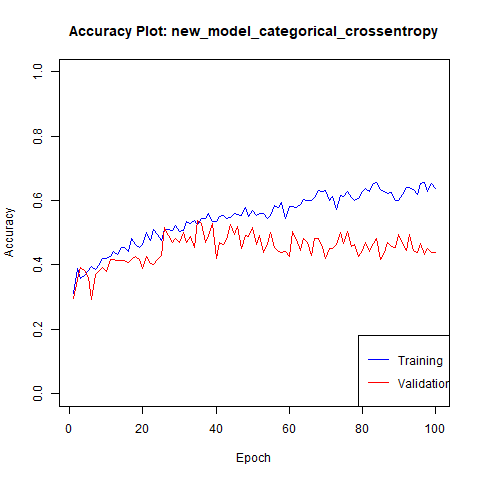
\includegraphics[width=0.8\textwidth]{../results/new_model_categorical_crossentropy_accuracy_plot.png}
    \caption{Model 2: Categorical Crossentropy Accuracy Over Epochs}
\end{figure}

The results were slightly better than the reduced dropout rate model but still indicated issues with generalization.

\section*{Discussion and Observations}

\subsection*{Comparison of Models Summary}
1. **Original Model (Day 1)**:
   - Showed steady improvement in training accuracy over 100 epochs.
   - Validation accuracy was erratic, indicating overfitting.

2. **Model 1 (Reduced Dropout Rate)**:
   - Slight improvement in training accuracy and validation accuracy. Not where I want it to be

3. **Model 2 (\texttt{categorical\_crossentropy})**:
   - Changing the loss function did not lead to an improvement

\subsection*{Key Observations}
The models performed poorly overall. Below are examples of correctly classified and misclassified images, I don't see a reason why this model did not get those right. Moving forward, I plan to explore image preprocessing techniques, as observed in Dan's work with the same dataset for CNNs, to improve results.

\begin{figure}[h!]
    \centering
    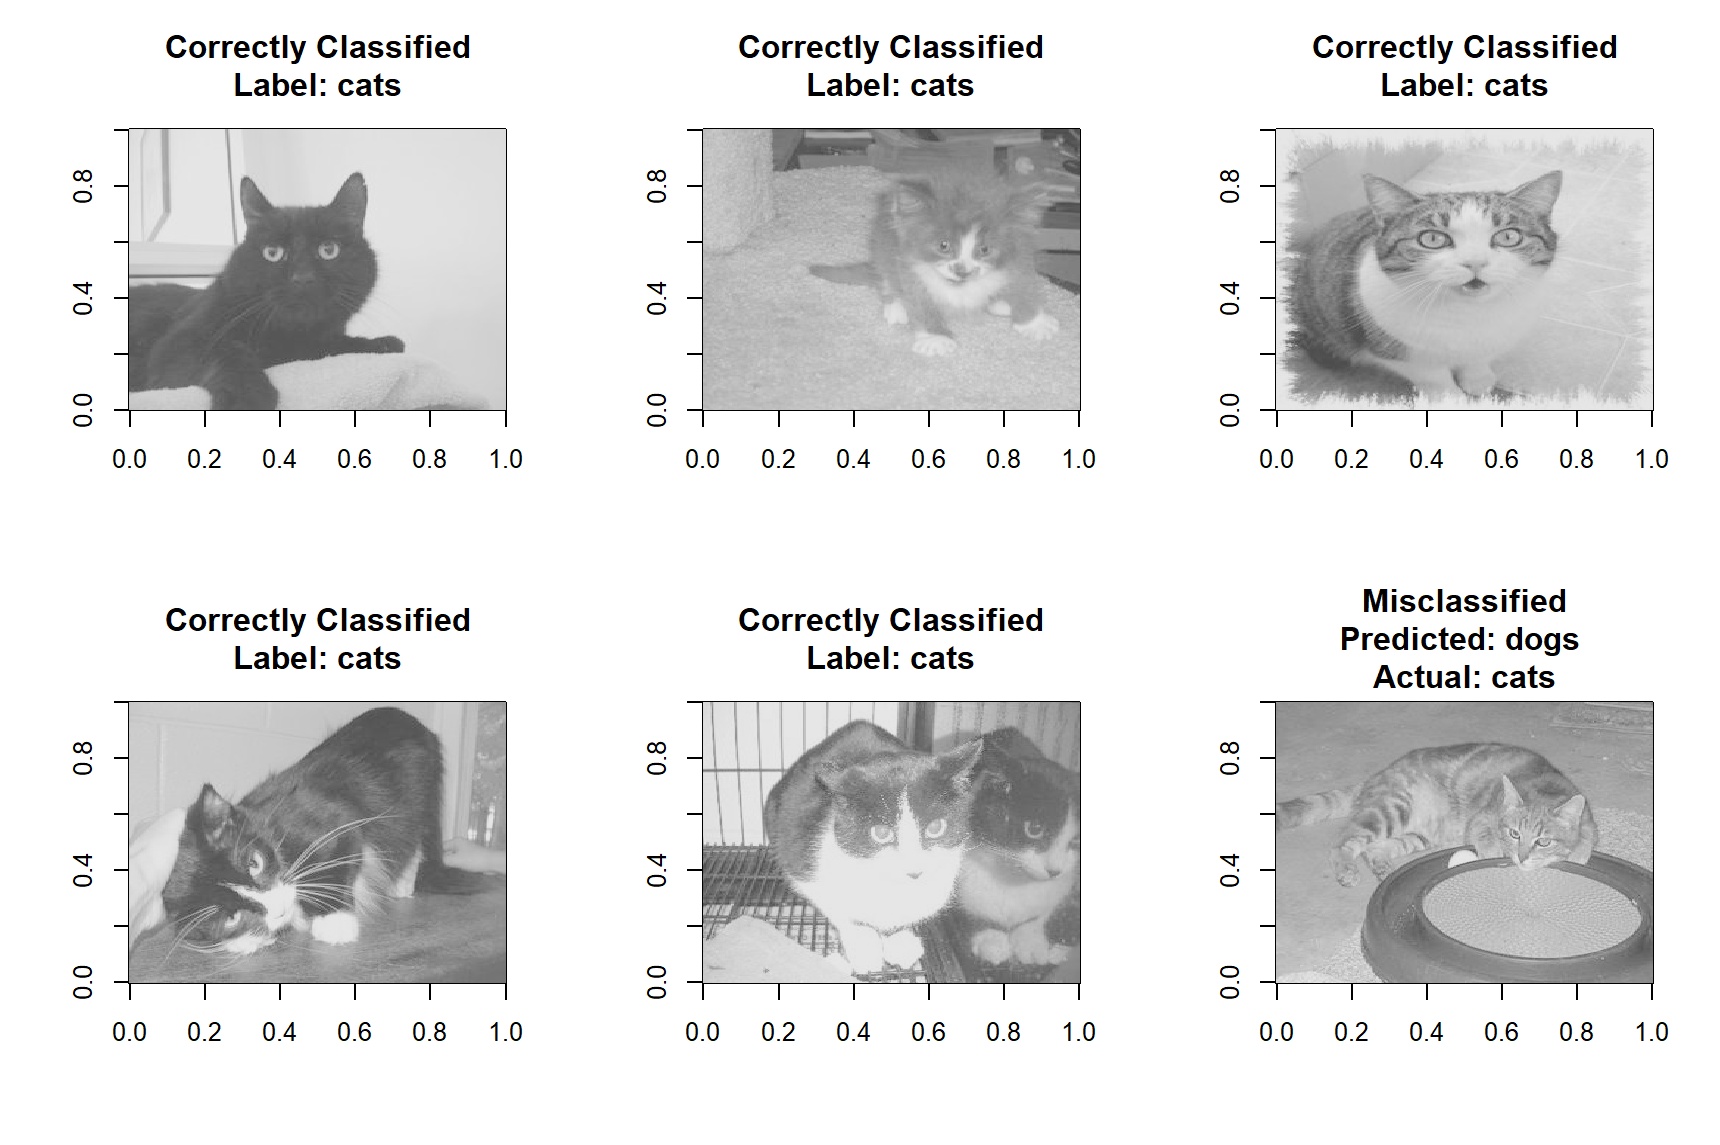
\includegraphics[width=0.8\textwidth]{../results/classified_examples.png}
    \caption{Examples of Correctly Classified Images}
\end{figure}

\begin{figure}[h!]
    \centering
    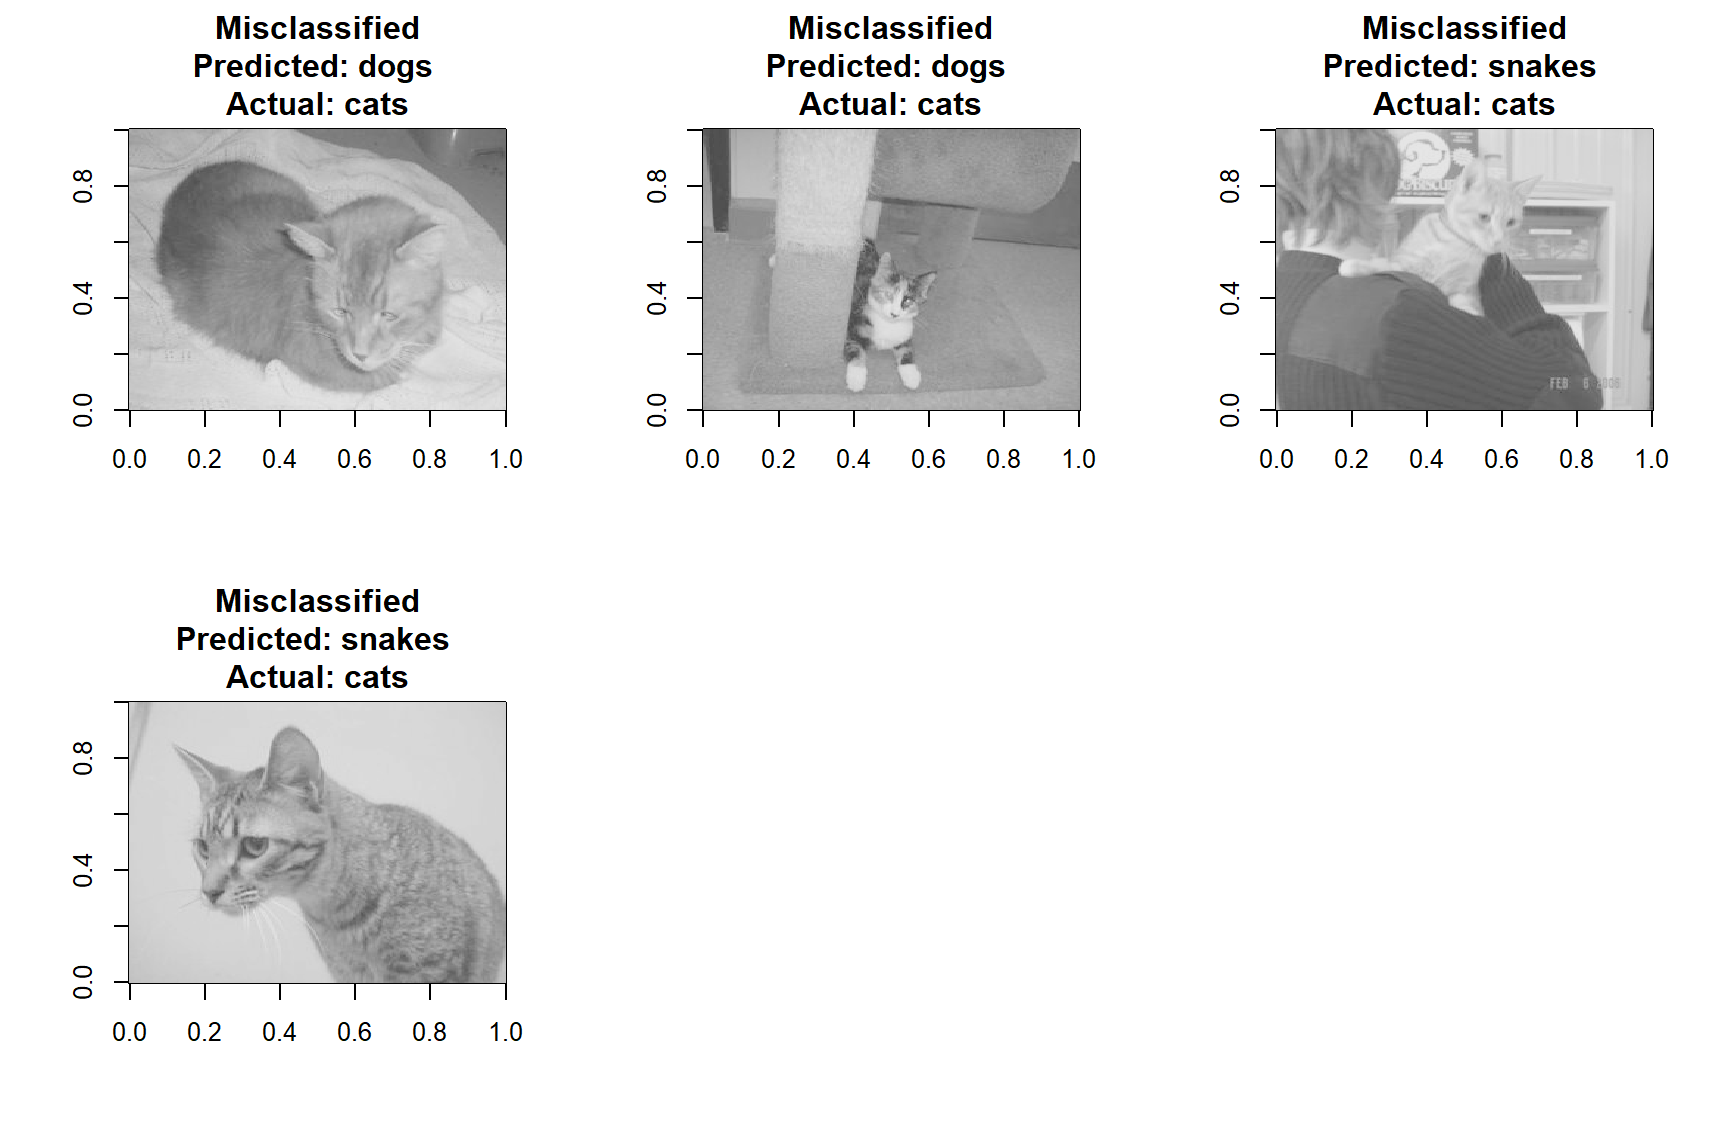
\includegraphics[width=0.8\textwidth]{../results/classified_images2.png}
    \caption{Examples of Misclassified Images}
\end{figure}

\section{Day 03 and 4: Convolutional Network}
I processed the data in the way I saw you do it in class. I think this helped a lot, as it kept the images in color. I got way better perfromance with the below models:


\subsection{Model 1: Simple CNN}
Model 1 is the simplest of the three architectures, designed as a baseline. The code for Model 1 is shown below:

\begin{verbatim}
model_1 <- keras_model_sequential() %>%
  layer_conv_2d(filters = 32, kernel_size = c(3, 3), activation = 'relu', input_shape = c(256, 256, 3)) %>%
  layer_max_pooling_2d(pool_size = c(2, 2)) %>%
  layer_flatten() %>%
  layer_dense(units = 128, activation = 'relu') %>%
  layer_dense(units = 3, activation = 'softmax')

model_1 %>% compile(
  optimizer = 'adam',
  loss = 'categorical_crossentropy',
  metrics = c('accuracy')
)
\end{verbatim}

This model uses the \texttt{Adam} optimizer.

\subsection{Model 2: Larger CNN with Additional Layers}
Model 2 introduces more complexity with more layers:


\begin{verbatim}
model_2 <- keras_model_sequential() %>%
  layer_conv_2d(filters = 64, kernel_size = c(3, 3), activation = 'relu', input_shape = c(256, 256, 3)) %>%
  layer_max_pooling_2d(pool_size = c(2, 2)) %>%
  layer_conv_2d(filters = 128, kernel_size = c(3, 3), activation = 'relu') %>%
  layer_max_pooling_2d(pool_size = c(2, 2)) %>%
  layer_flatten() %>%
  layer_dense(units = 256, activation = 'relu') %>%
  layer_dense(units = 3, activation = 'softmax')

model_2 %>% compile(
  optimizer = 'sgd',
  loss = 'categorical_crossentropy',
  metrics = c('accuracy')
)
\end{verbatim}

This model uses the \texttt{SGD} (Stochastic Gradient Descent) optimizer, which "updates weights incrementally and is known for its stability." 

\subsection{Model 3: CNN with Dropout Regularization}
Model 3 incorporates dropout layers for regularization:

\begin{verbatim}
model_3 <- keras_model_sequential() %>%
  layer_conv_2d(filters = 64, kernel_size = c(3, 3), activation = 'relu', input_shape = c(256, 256, 3)) %>%
  layer_max_pooling_2d(pool_size = c(2, 2)) %>%
  layer_dropout(rate = 0.25) %>%
  layer_conv_2d(filters = 128, kernel_size = c(3, 3), activation = 'relu') %>%
  layer_max_pooling_2d(pool_size = c(2, 2)) %>%
  layer_dropout(rate = 0.5) %>%
  layer_flatten() %>%
  layer_dense(units = 512, activation = 'relu') %>%
  layer_dense(units = 3, activation = 'softmax')

model_3 %>% compile(
  optimizer = 'rmsprop',
  loss = 'categorical_crossentropy',
  metrics = c('accuracy')
)
\end{verbatim}

This model utilizes the \texttt{RMSprop} optimizer, which "divides the learning rate by a moving average of the magnitudes of recent gradients."



\subsection{Model 1 Performance}

\begin{figure}[h!]
    \centering
    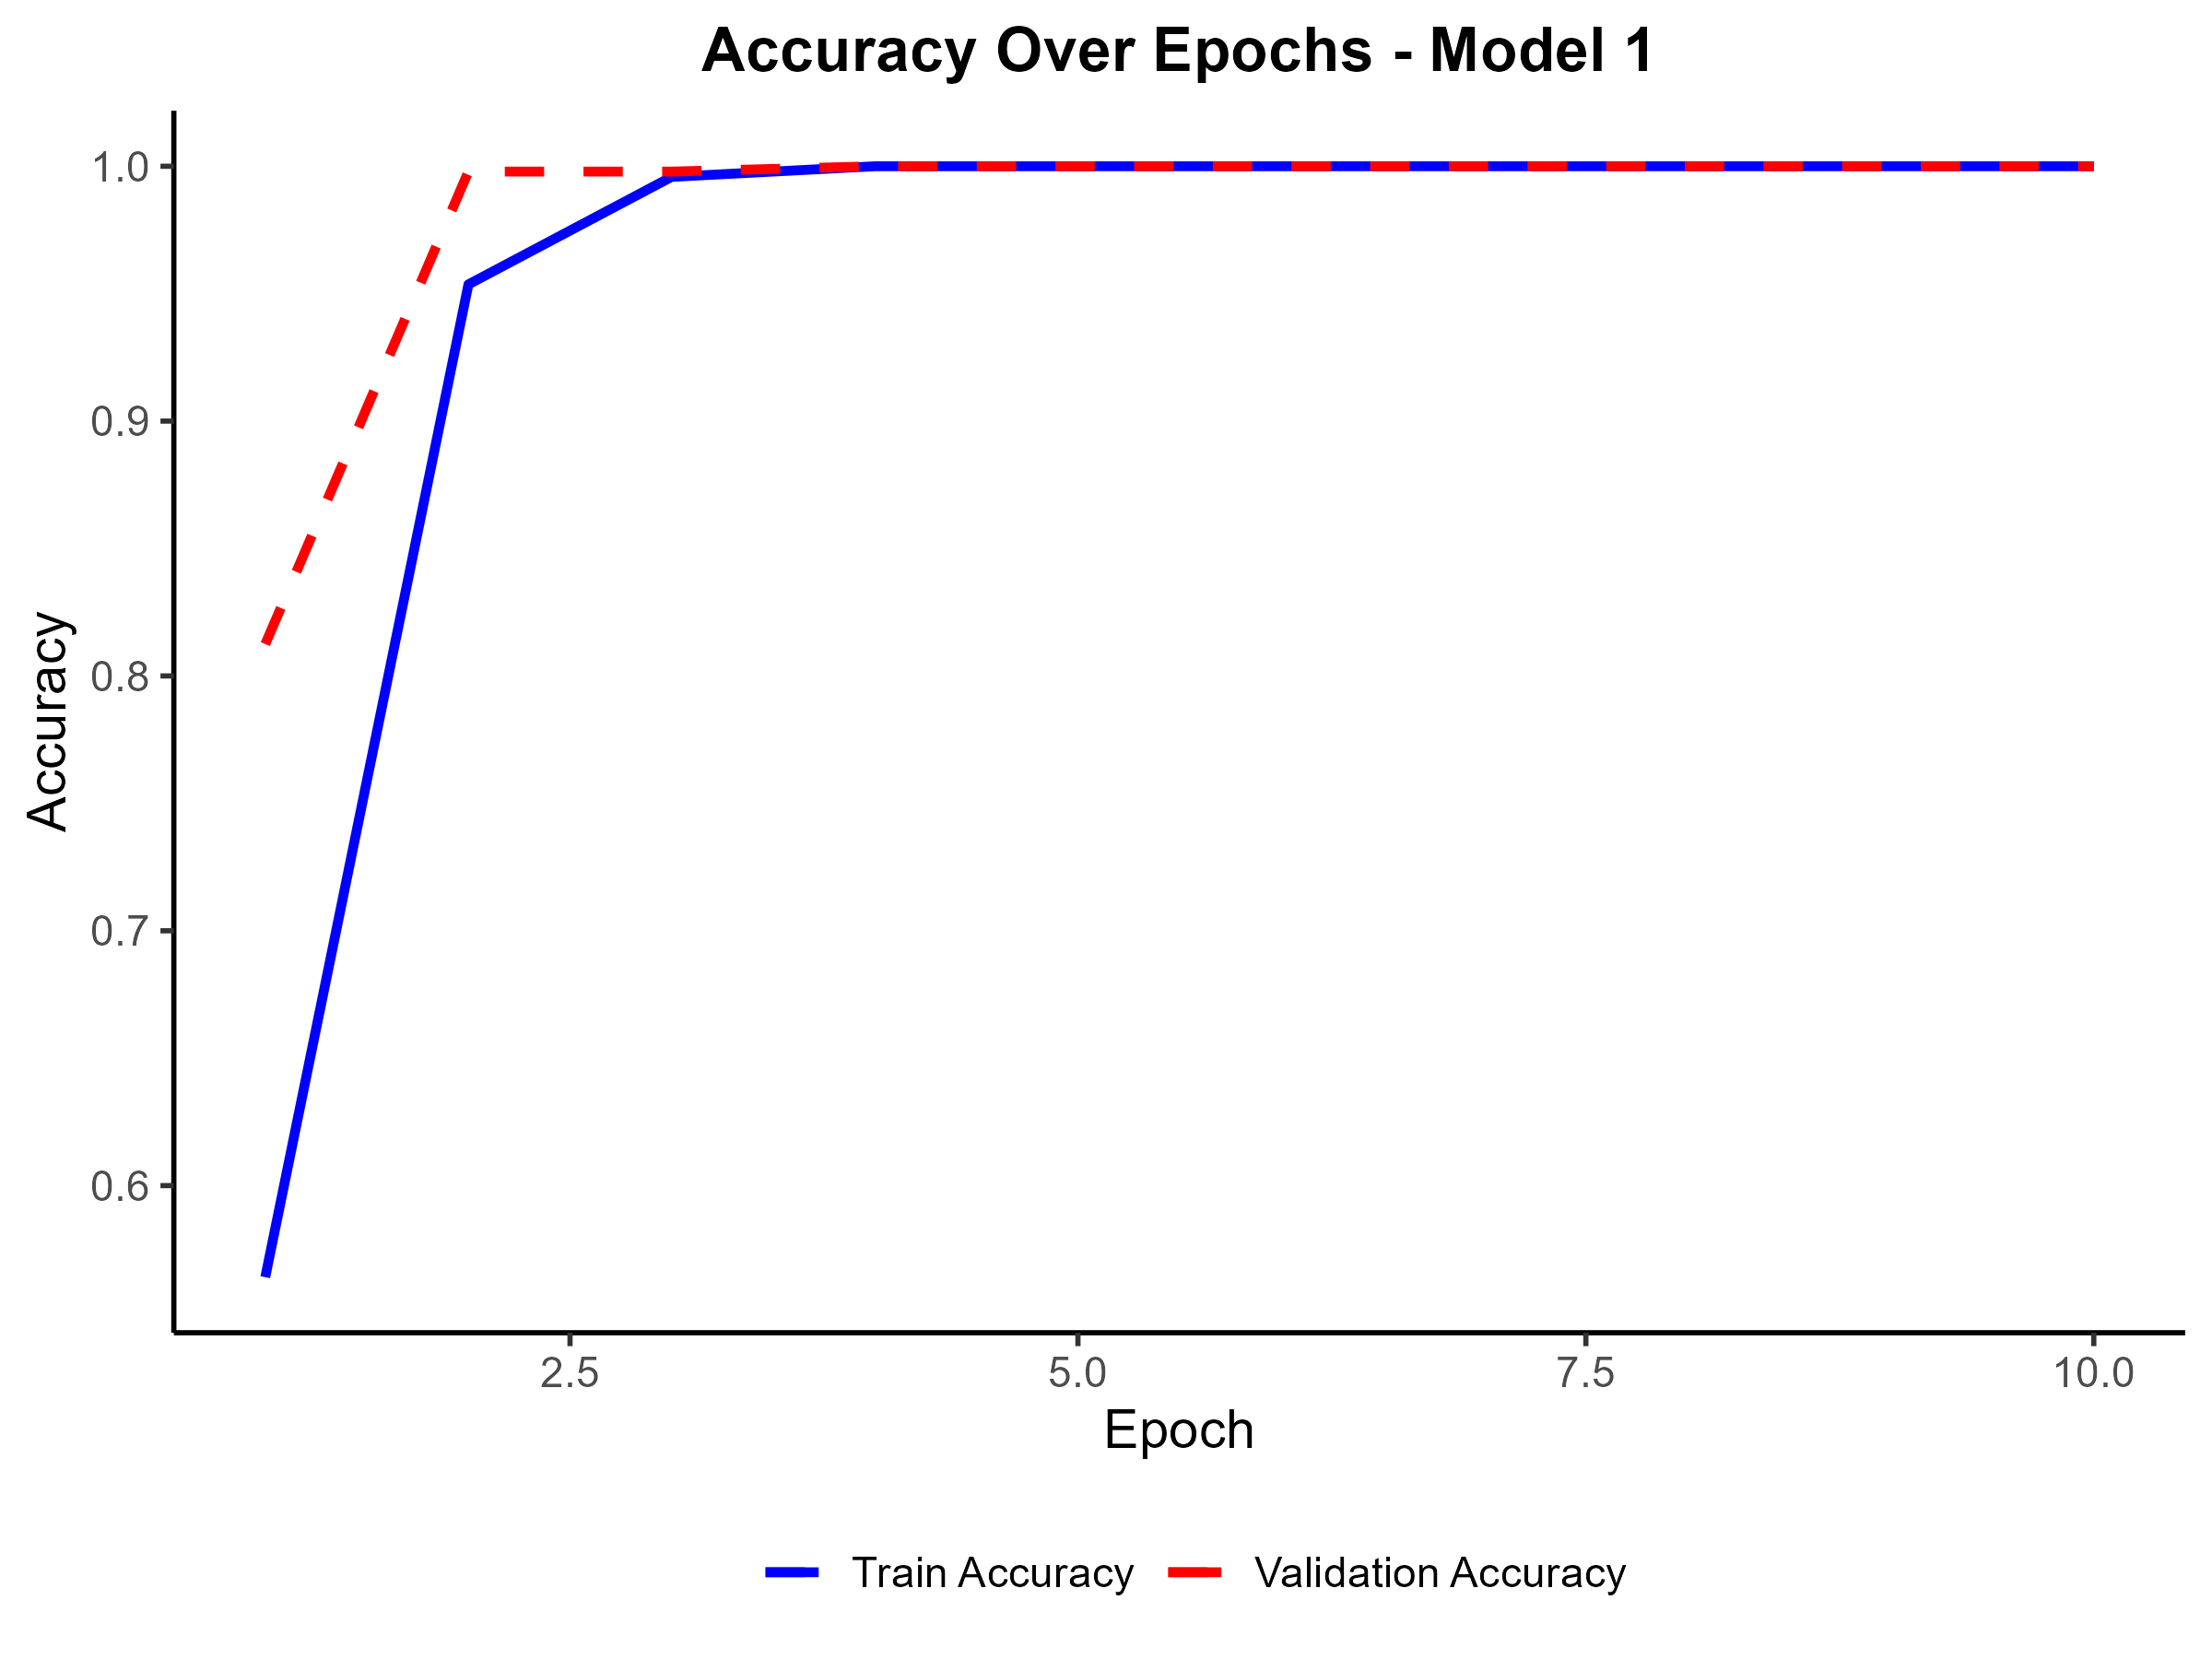
\includegraphics[width=0.6\textwidth]{../results/accuracy_plot_model_1.png}
    \caption{Accuracy trends for Model 1. Train accuracy is shown in blue, and validation accuracy is shown in red.}
    \label{fig:model1}
\end{figure}

\subsection{Model 2 Performance}
Model 2 also showed improvements in training accuracy but experienced significant fluctuations in validation accuracy. I'm not sure why it is such a sharp increase and decrease in validation accuracy, but it eventually stabilizes!

\begin{figure}[H]
    \centering
    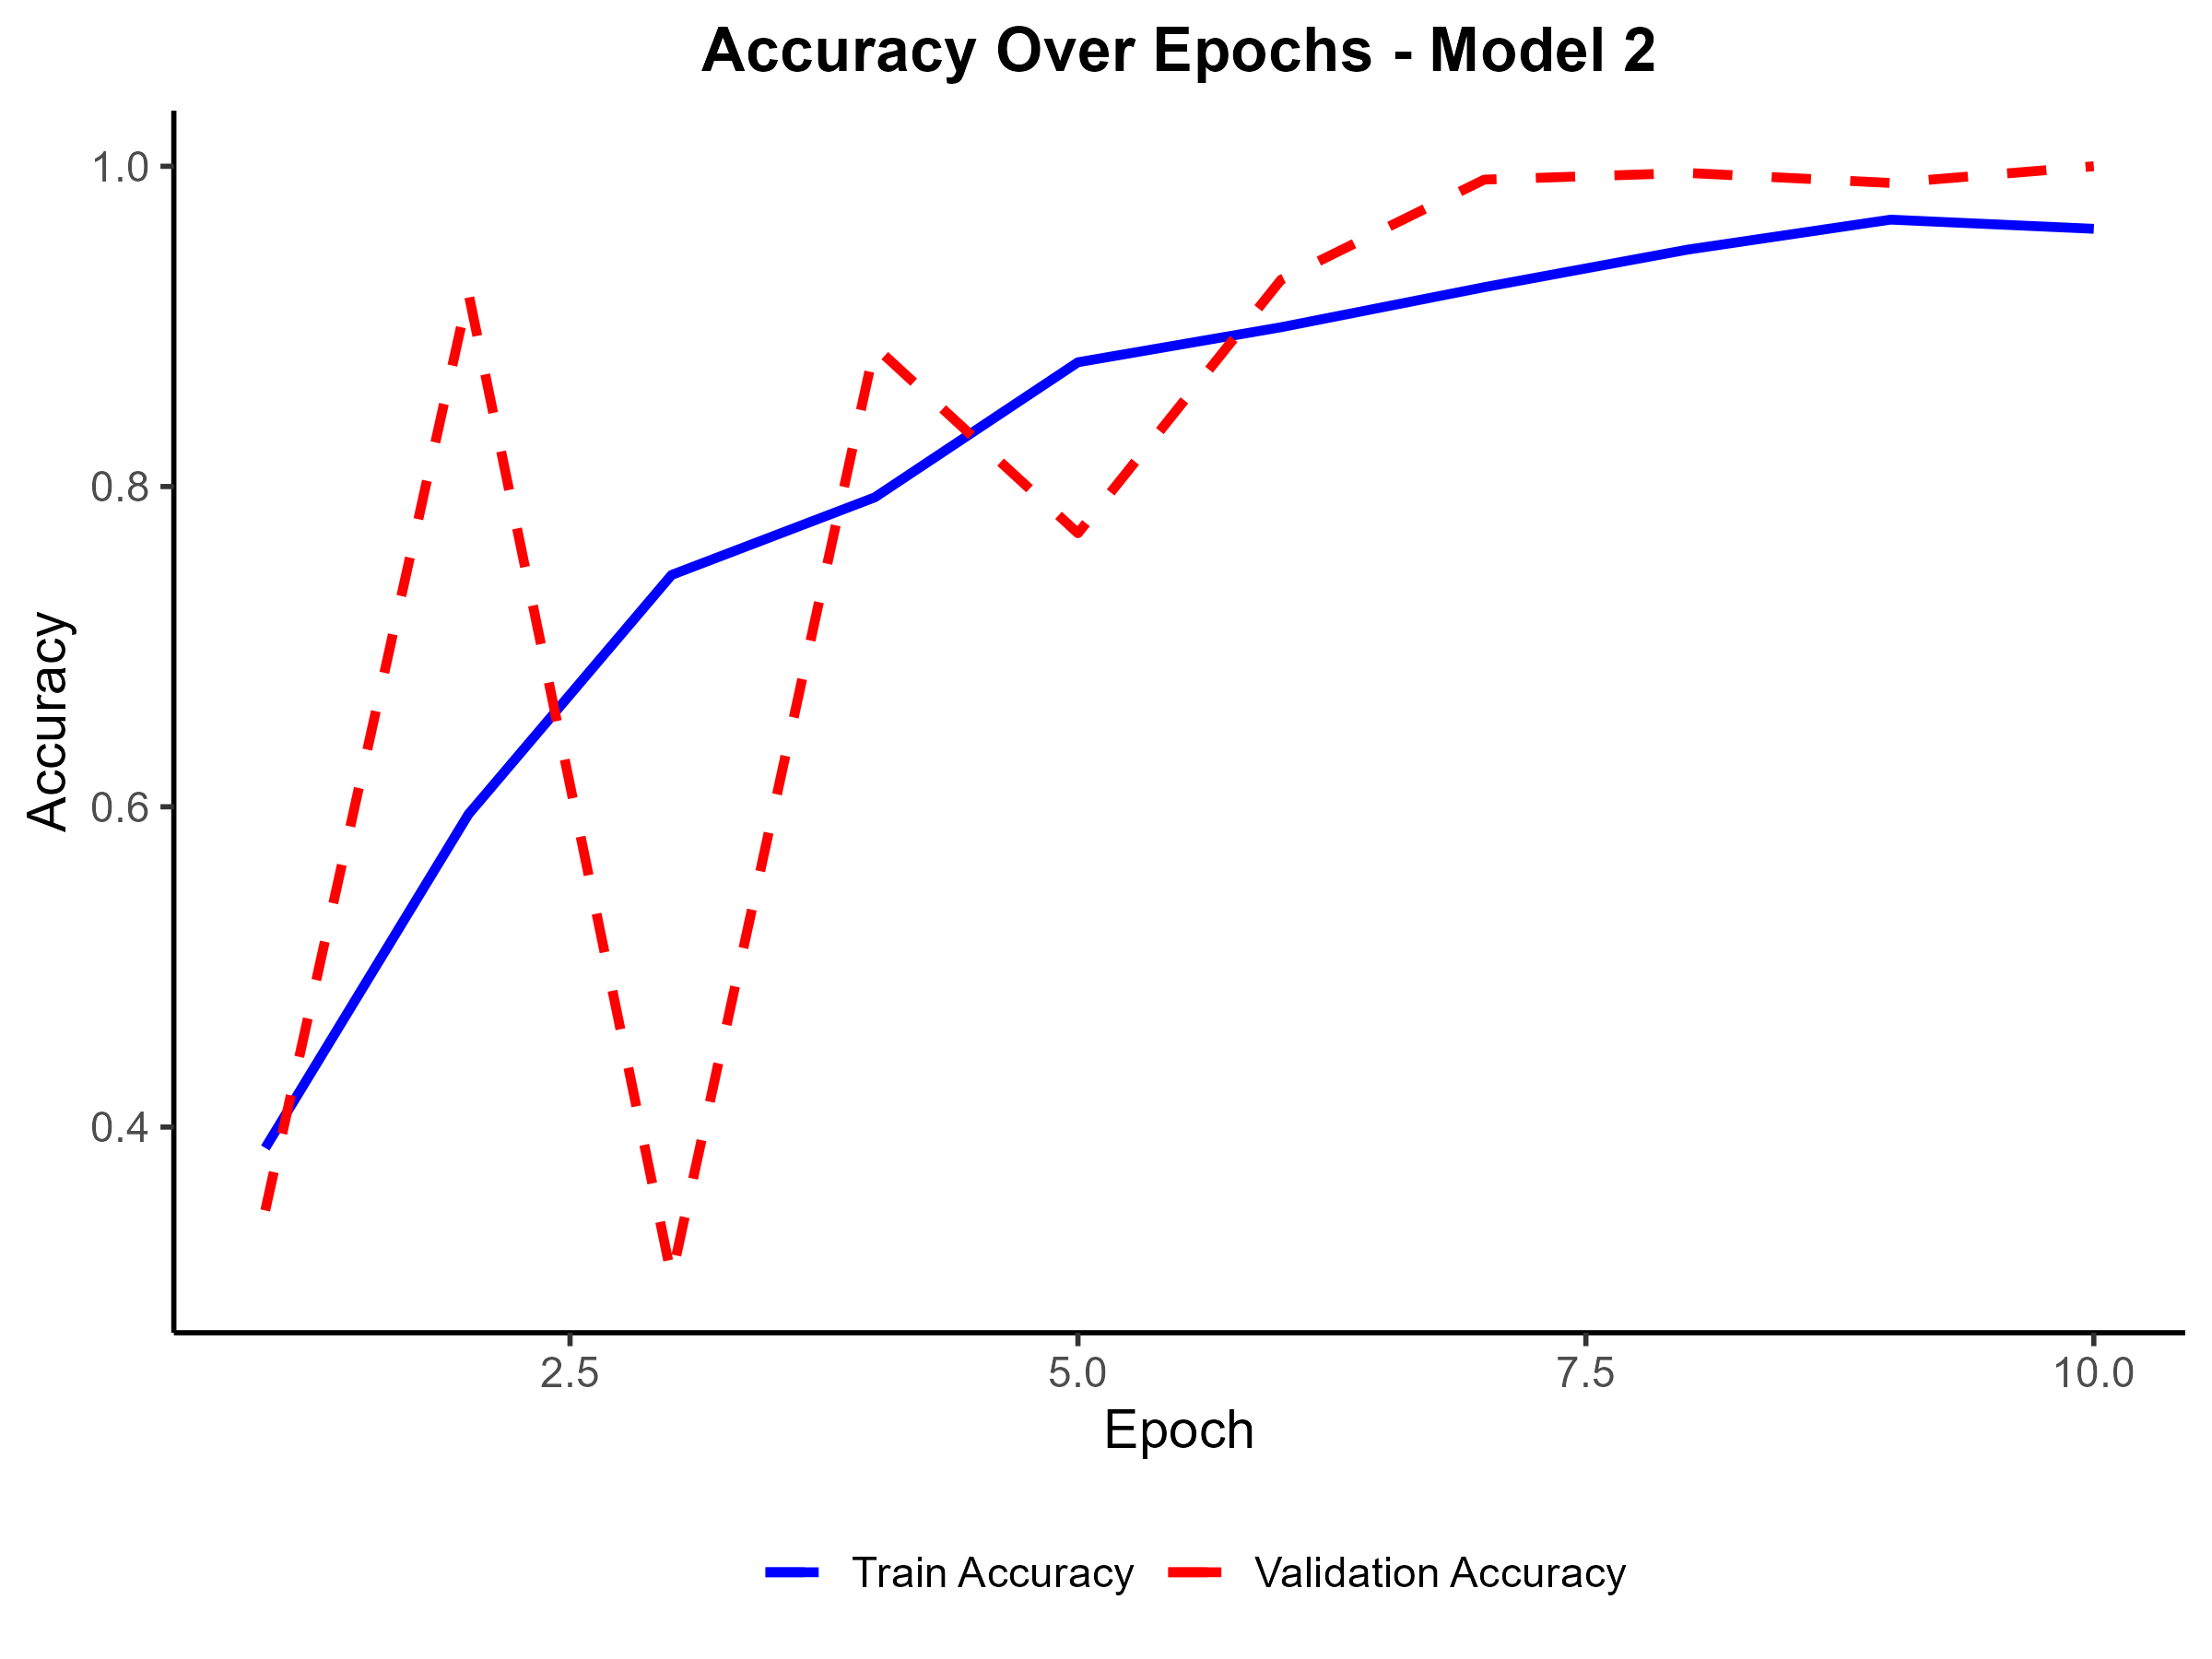
\includegraphics[width=0.6\textwidth]{../results/accuracy_plot_model_2.png}
    \caption{Accuracy trends for Model 2. Train accuracy is shown in blue, and validation accuracy is shown in red.}
    \label{fig:model2}
\end{figure}

\subsection{Model 3 Performance}
Model 3 underperformed compared to the other models. Both train and validation accuracies remained low, indicating strong regularization effects due to the dropout layers, possibly leading to underfitting. I also think if I ran this for more epochs it could have done better, but still it likely wouldn't outperform model 1. 

\begin{figure}[h!]
    \centering
    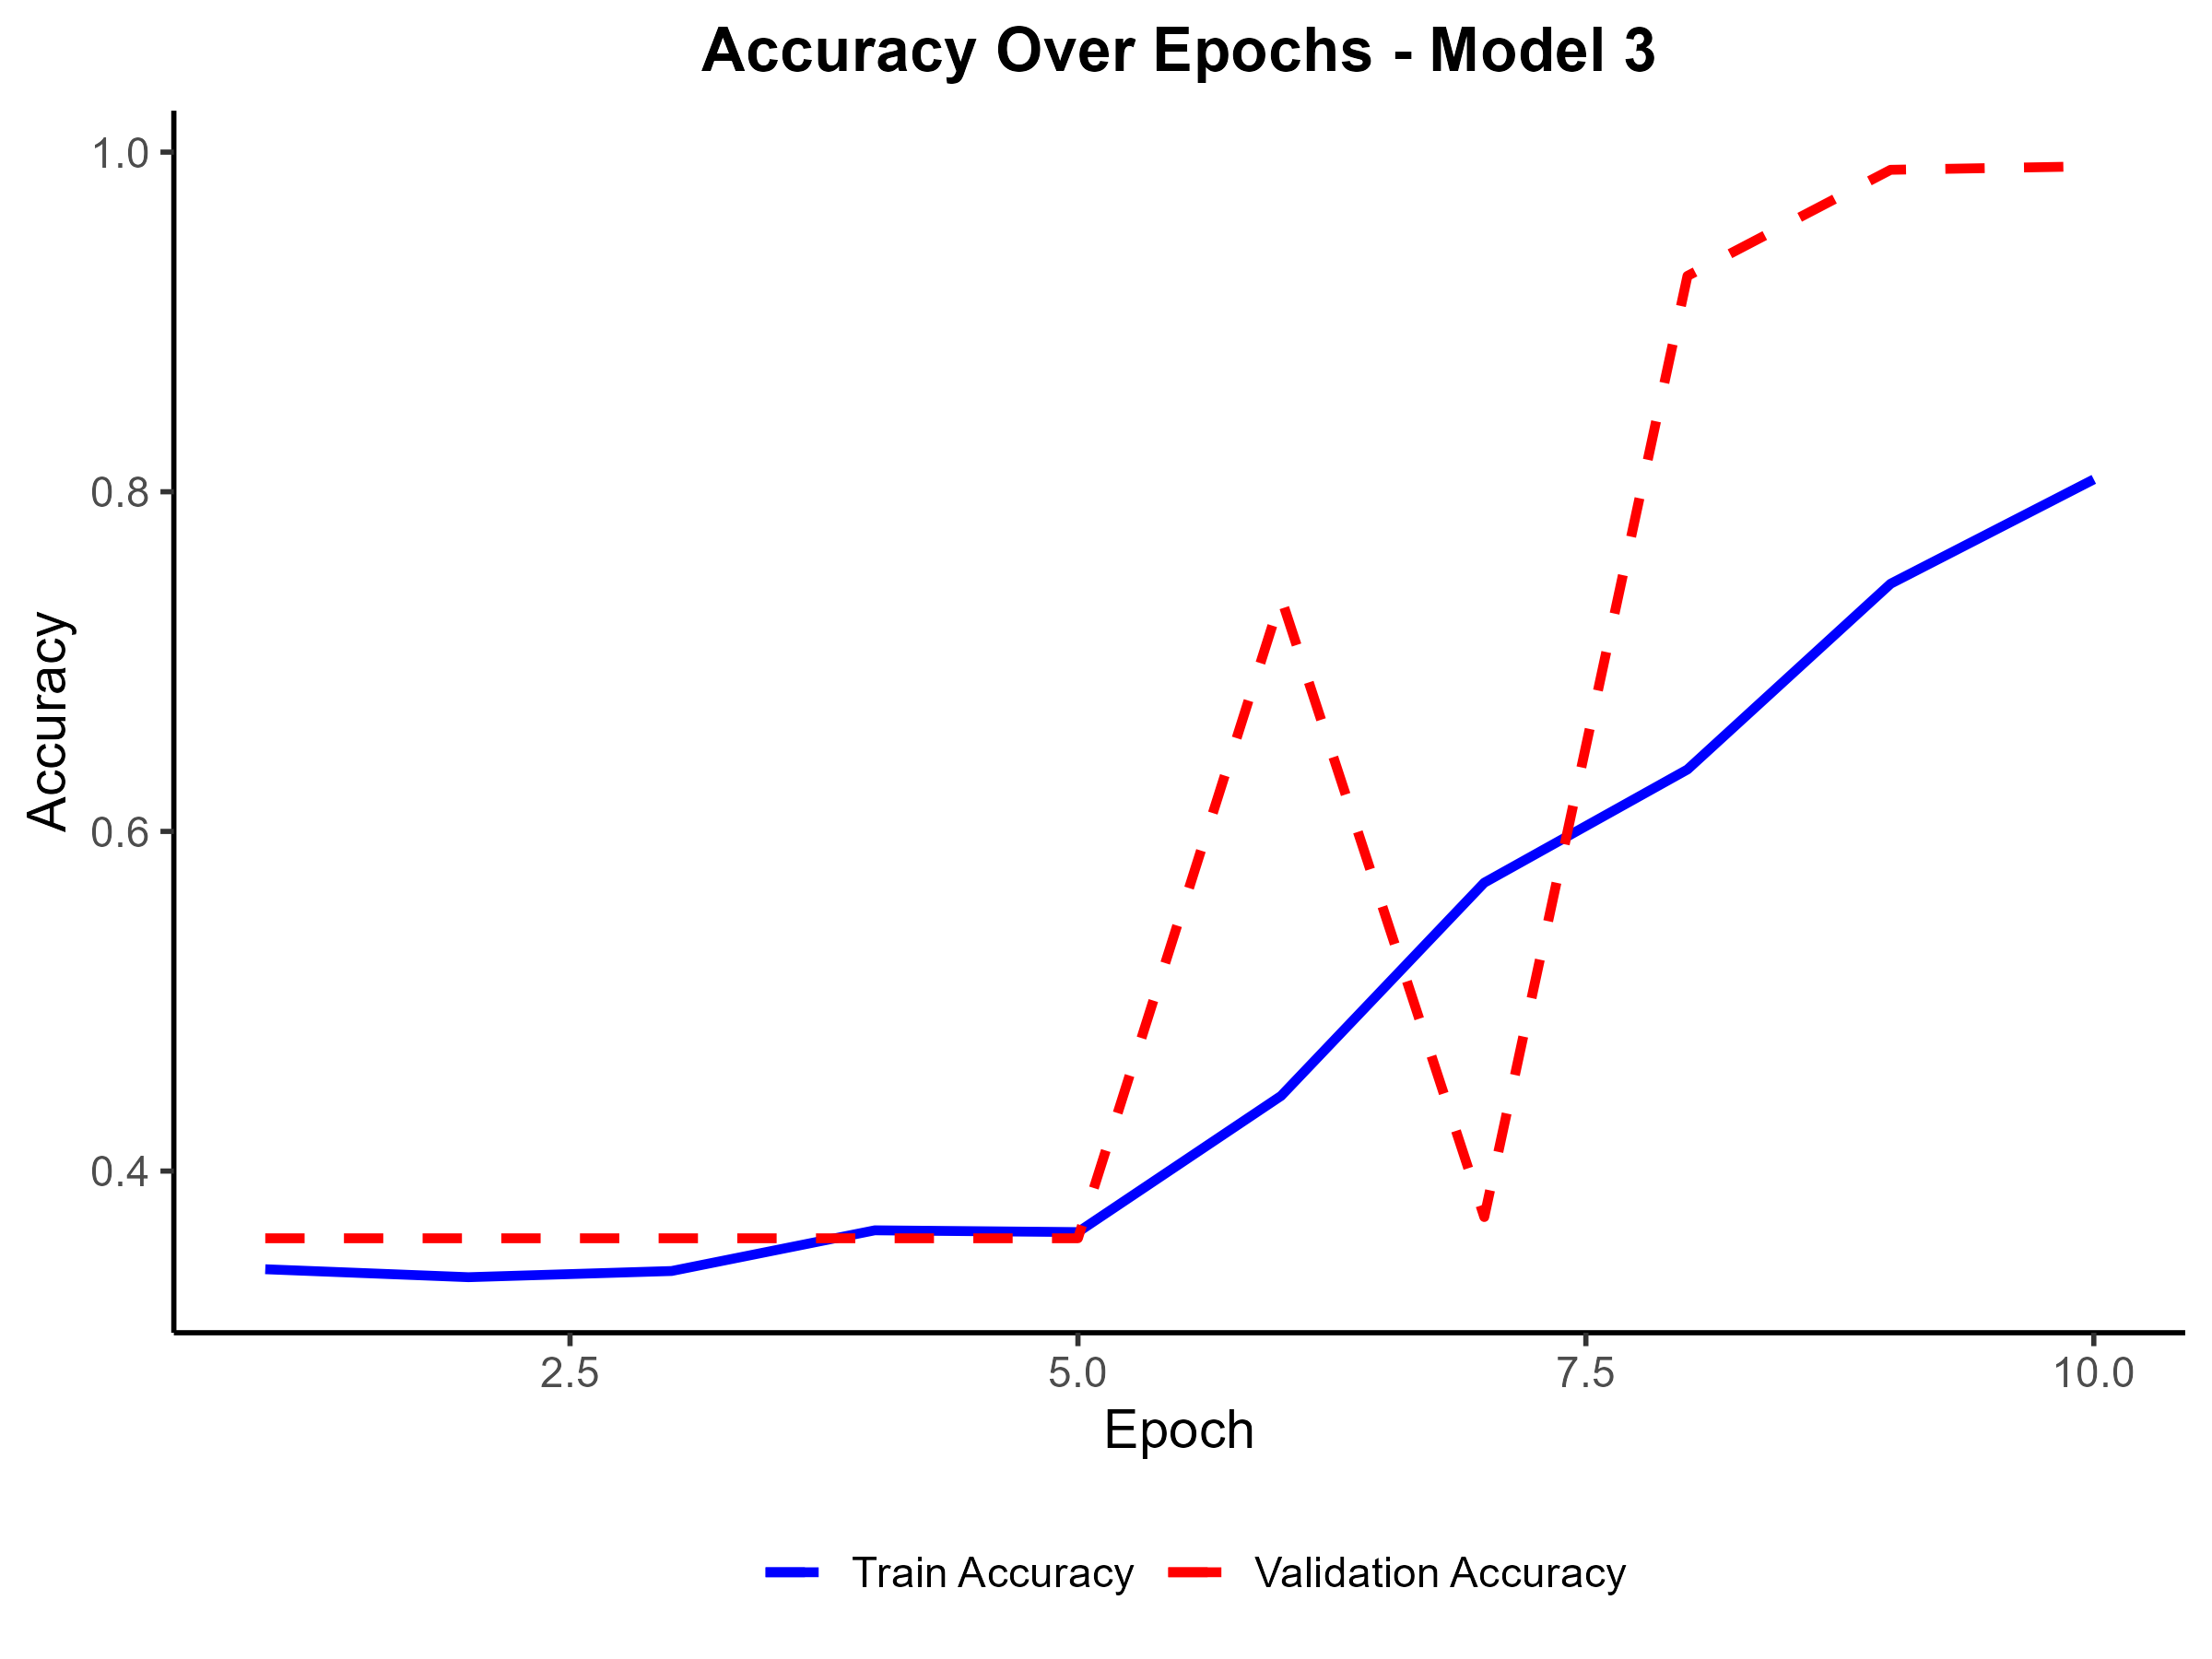
\includegraphics[width=0.6\textwidth]{../results/accuracy_plot_model_3.png}
    \caption{Accuracy trends for Model 3. Train accuracy is shown in blue, and validation accuracy is shown in red.}
    \label{fig:model3}
\end{figure}


\begin{table}[H]
\centering
\caption{Test Accuracy of Different Models from Day 3-4}
\label{tab:model_accuracy}
\begin{tabular}{|c|c|}
\hline
\textbf{Model} & \textbf{Test Accuracy} \\ \hline
Model 1 (Simple CNN)       & 1.000       \\ \hline
Model 2 (Larger CNN)       & 0.748       \\ \hline
Model 3 (CNN with Dropout) & 0.998       \\ \hline
\end{tabular}
\end{table}

It looks like Model 1 is the best. it correctly predicted all of the testing data.I will use it for comparison on transfer learning for Day5. 

\section{Day 5: Transfer Learning}
The pre-trained MobileNetV2 model was used as the base feature extractor, followed by a custom architecture similar to the previously best-performing model from Day3 and 4. The following code demonstrates the setup of the transfer learning model:

\begin{verbatim}
# Load MobileNetV2 pre-trained model without top layers
base_model <- application_mobilenet_v2(
  include_top = FALSE,          #Exclude original classifier
  weights = "imagenet",         #pre-trained ImageNet weights
  input_shape = c(256, 256, 3)  #match input shape from before
)

#cool freeze weights function
freeze_weights(base_model)

#Build the transfer learning model
transfer_model <- keras_model_sequential() %>%
  base_model %>%
  layer_conv_2d(filters = 32, kernel_size = c(3, 3), activation = 'relu') %>%
  layer_max_pooling_2d(pool_size = c(2, 2)) %>%
  layer_flatten() %>%
  layer_dense(units = 128, activation = 'relu') %>%
  layer_dense(units = 3, activation = 'softmax')

#compile
transfer_model %>% compile(
  optimizer = 'adam',
  loss = 'categorical_crossentropy',
  metrics = c('accuracy')
)
\end{verbatim}

\section{Training and Evaluation}
The transfer learning model was trained using the same training and testing datasets as in Day 3. The training process spanned 10 epochs, with a batch size of 32:

\begin{verbatim}
# Train the model
history_transfer <- transfer_model %>% fit(
  x = x_train,
  y = y_train,
  epochs = 10,
  batch_size = 32,
  validation_data = list(x_test, y_test)
)

#Evaluate the model
test_eval <- transfer_model %>% evaluate(x_test, y_test)
\end{verbatim}

The transfer model's accuracy was compared to the previous best-performing model's accuracy from Day 3 and 4 (Model 1). This was the most simple model, and its' accuracy could not really be beat. 

\section{Results}

\subsection{Accuracy Plot}
The training and validation accuracy trends for the transfer learning model are shown in Figure~\ref{fig:transfer-accuracy}.

\begin{figure}[h!]
    \centering
    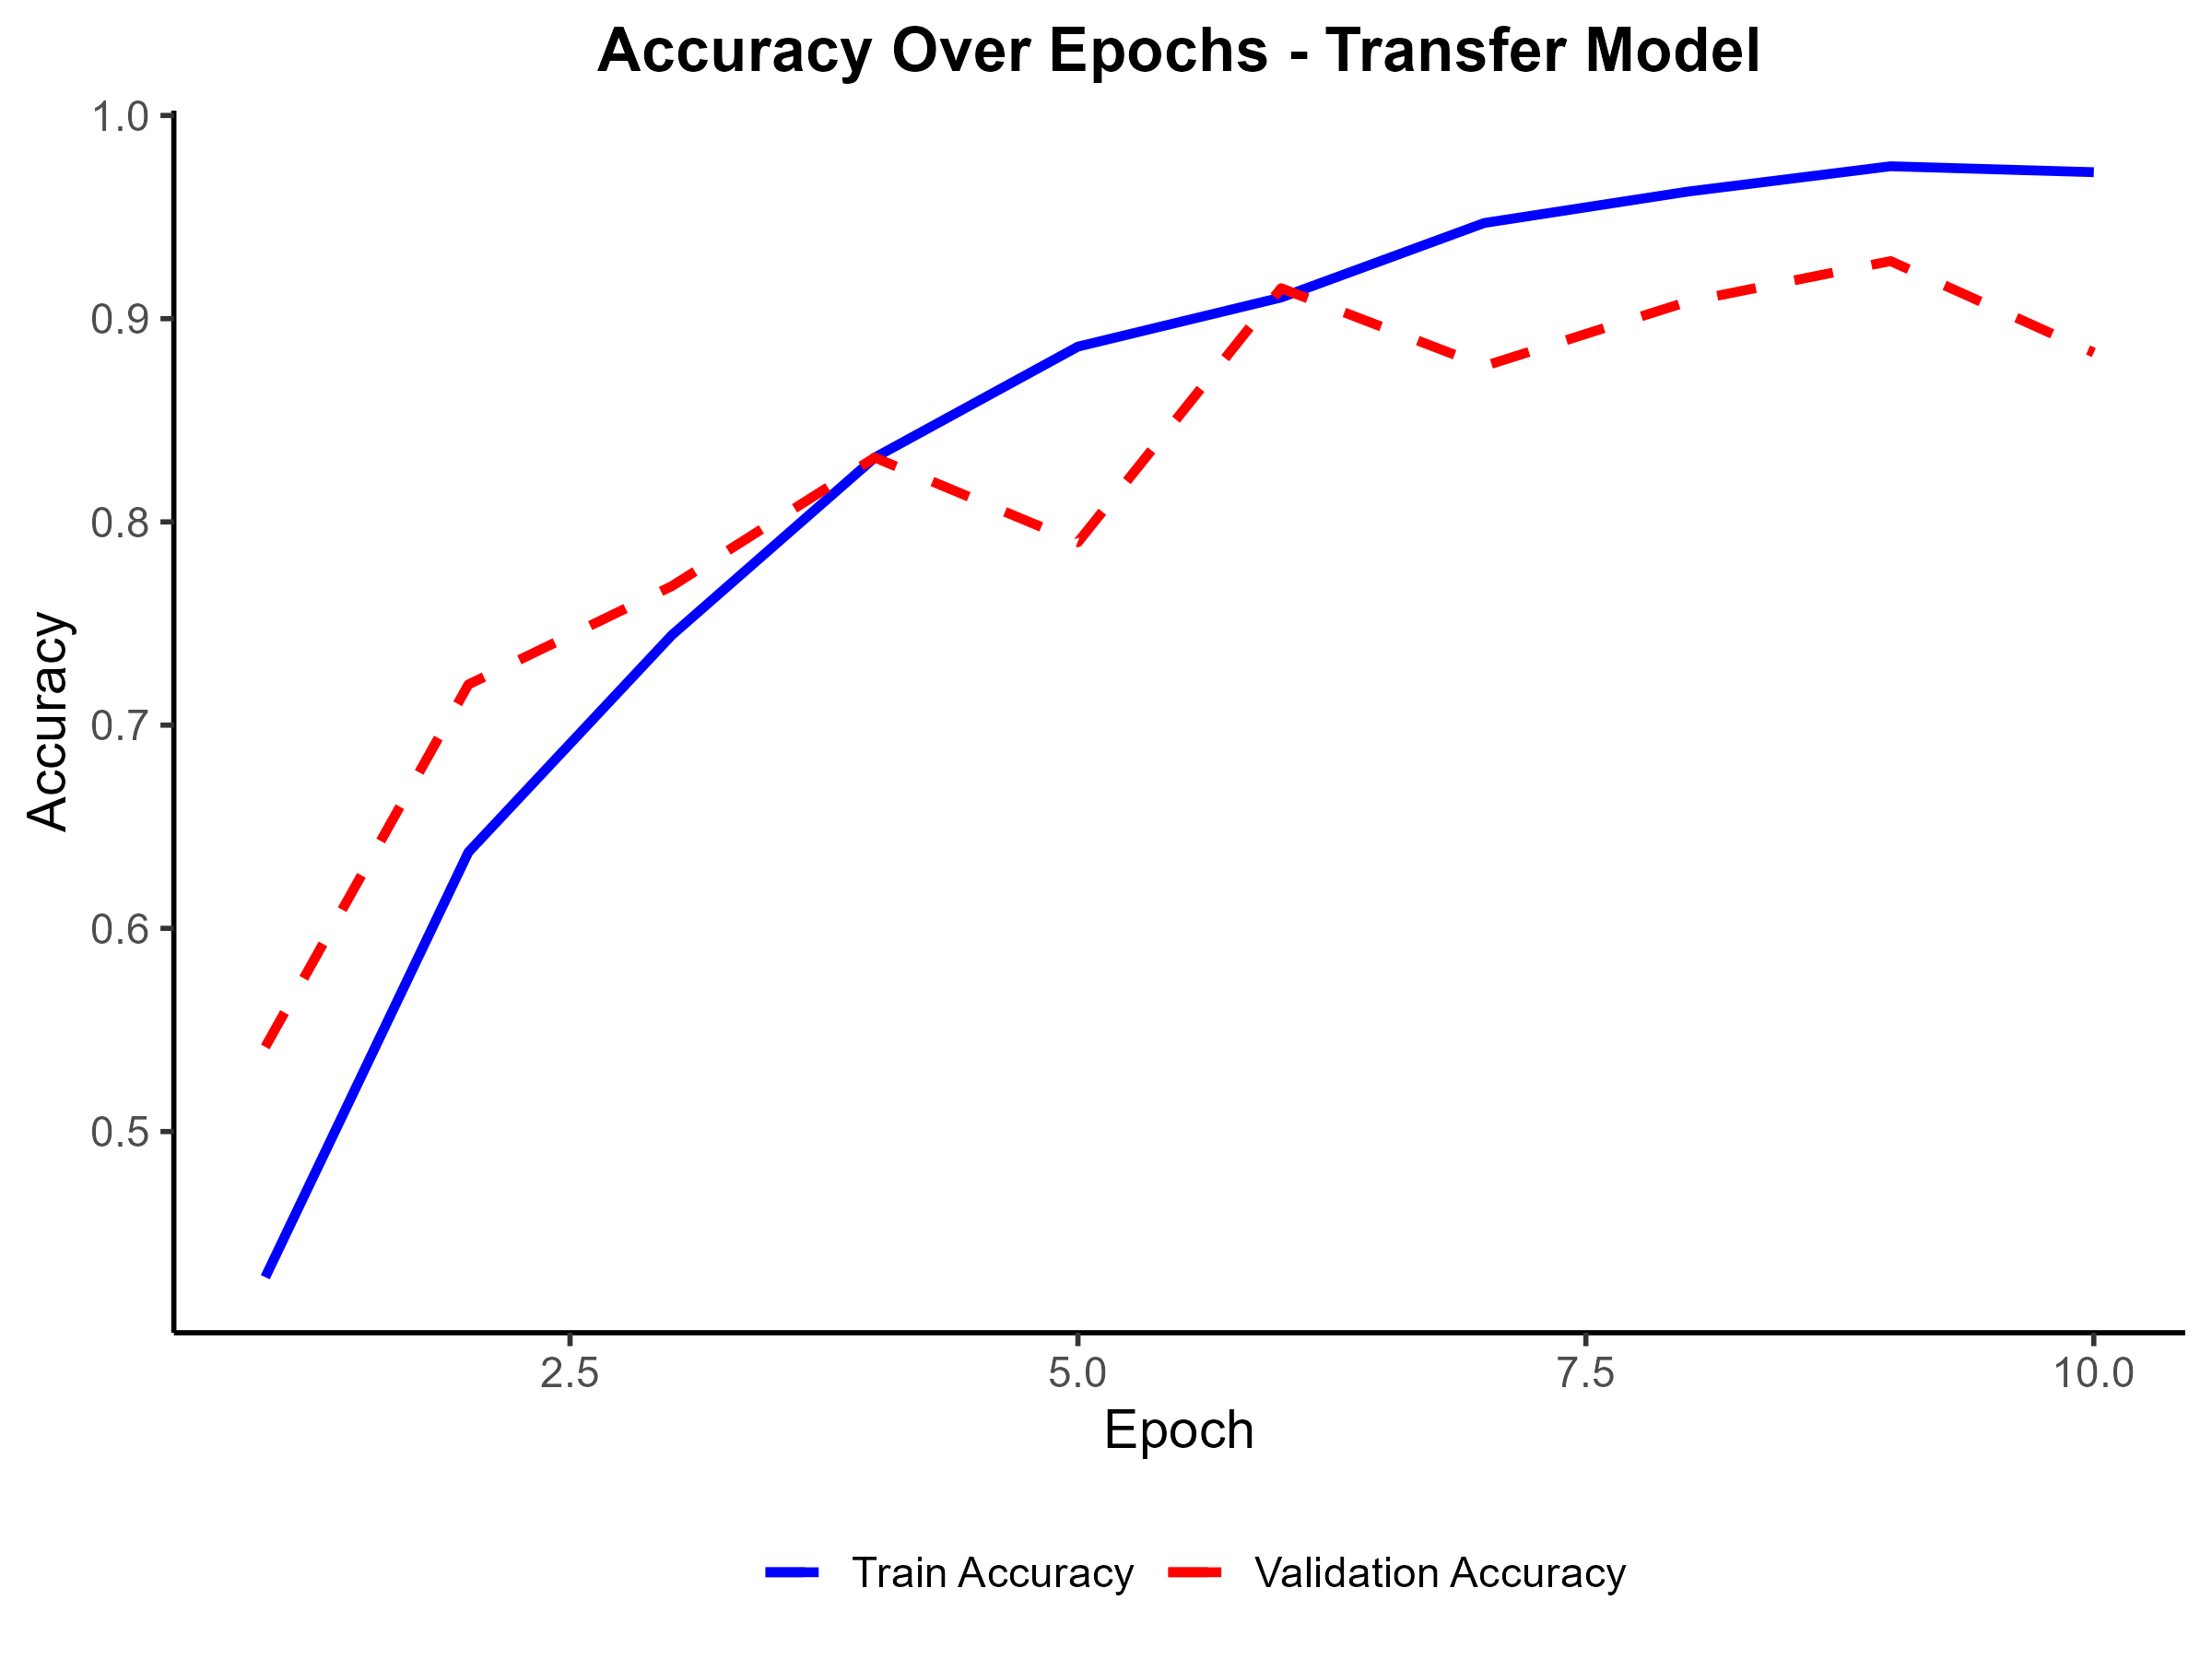
\includegraphics[width=0.8\textwidth]{../results/transfer_model_accuracy.png}
    \caption{Accuracy trends for the transfer learning model. Train accuracy is shown in blue, and validation accuracy is shown in red.}
    \label{fig:transfer-accuracy}
\end{figure}

\subsection{Accuracy Comparison}
Table~\ref{tab:accuracy} compares the test accuracy of the transfer learning model with the best-performing model (Model 1) from Day 3. I don't think I am surprised by this, as the more complicated models the other day did not do as well as the simple one, so these pretrained models online were to complex for this "simple" classification problem. The simple model was probably more effective for this specific dataset because it had smaller and more task-oriented architecture that would have allowed it to focus on learning the problem features directly without having to first relearn pre-trained weights? 

\begin{table}[h!]
    \centering
    \begin{tabular}{l c}
        \hline
        \textbf{Model} & \textbf{Test Accuracy} \\
        \hline
        Transfer Learning Model & 0.91667 \\
        Best Model (Day 3)      & 1.0000 \\
        \hline
    \end{tabular}
    \caption{comparisons}
    \label{tab:accuracy}
\end{table}


\end{document}


